\documentclass[11pt]{article}

\usepackage[margin=1.7cm,top=2.5cm,bottom=2cm,letterpaper]{geometry}
\usepackage{enumitem}
\usepackage{tikz}
\usepackage{mathpazo}
\usepackage{times}
\usepackage[document]{ragged2e}
\usepackage[none]{hyphenat}
\usepackage{siunitx}
\usepackage[siunitx]{circuitikz}
\usepackage{multicol}
\usepackage{fancyhdr}

\sisetup{number-math-rm=\mathnormal}

\newcommand{\pic}[2]{\includegraphics[width=#1\textwidth]{#2}}

\setlength{\parindent}{0pt}
\setlength{\headheight}{14pt}


\begin{document}

\pagestyle{fancy}
\rhead{Name:\hspace{1.5in}Student Number:\hspace{.75in}}
\chead{}
\lhead{Olympiads School}
\lfoot{}\cfoot{-\textsf{\textbf{\thepage}}-}
\rfoot{\textsf{\textbf{GO ON TO THE NEXT PAGE.}}}

\begin{center}
  \vspace{-.35in}
  {\large
    \textbf{AP PHYSICS C: CIRCUIT ANALYSIS}
  }
\end{center}

\textbf{Directions:} Each of the questions or incomplete statements below is
followed by five suggested answers or\\
completions. Select the one that is best
in each case and place the letter of your choice in the corresponding box on
the student answer sheet.

\vspace{10pt}\textbf{Note:} To simplify calculations, you may use
$g=\SI{10}{m/s^2}$ in all problems.

\raggedcolumns
\begin{multicols}{2}
%  \begin{enumerate}[leftmargin=18pt]
%
%  \item Two electric objects experience a repulsive force. What happens to that
%    force if the distance between the objects is doubled?
%    \begin{enumerate}[noitemsep,topsep=0pt,leftmargin=18pt,label=(\Alph*)]
%    \item It decreases to one-fourth its value.
%    \item It decreases to one-half its value.
%    \item It stays the same.
%    \item It doubles.
%    \item It quadruples.
%    \end{enumerate}
%
%  \item A pith ball is a tiny piece of Styrofoam that is covered with a
%    conductive paint. One pith ball initially has a charge of \SI{6.4e-8}{C},
%    and it touches an identical, neutral pith ball. After the pith balls are
%    separated, what is the charge on the pith ball that had the initial charge?
%    \begin{enumerate}[noitemsep,topsep=0pt,leftmargin=18pt,label=(\Alph*)]
%    \item\SI{6.4e-8}{C}
%    \item\SI{3.2e-8}{C}
%    \item\SI{0}{C}
%    \item\SI{-3.2e-8}{C}
%    \item\SI{-6.4e-8}{C}
%    \end{enumerate}
%
%  \item Glass becomes positively charged when it is rubbed with silk. Which
%    of the following is the best description of what’s happening?
%    \begin{enumerate}[noitemsep,topsep=0pt,leftmargin=18pt,label=(\Alph*)]
%    \item Electrons are rubbed off the glass onto the silk.
%    \item Electrons are rubbed off the silk onto the glass.
%    \item Protons are rubbed off the glass onto the silk.
%    \item Protons are rubbed off the silk onto the glass.
%    \item Neutrons in the glass have an affinity for positive charge.
%    \end{enumerate}
%  
%  \item Consider an isolated, neutral system consisting of wool fabric and a
%    rubber rod. If the rubber rod is rubbed with wool to become negatively
%    charged, what can be said about the wool fabric?
%    \begin{enumerate}[noitemsep,topsep=0pt,leftmargin=18pt,label=(\Alph*)]
%    \item It becomes equally negatively charged.
%    \item It becomes equally positively charged.
%    \item It becomes negatively charged but not equally.
%    \item It becomes positively charged but not equally.
%    \item In a neutral system, neither object can become charged.
%    \end{enumerate}
%    \columnbreak
%  \item An electron and a proton are separated by \SI{1.50e-10}{m}. If they are
%    released, which one will accelerate at a greater rate, and what is the
%    magnitude of that acceleration?
%    \begin{enumerate}[noitemsep,topsep=0pt,leftmargin=18pt,label=(\Alph*)]
%    \item The electron; \SI{1.12e22}{m/s^2}
%    \item The proton; \SI{1.12e22}{m/s^2}
%    \item The electron; \SI{6.13e18}{m/s^2}
%    \item The proton; \SI{6.13e18}{m/s^2}
%    \item They both accelerate at the same rate; \SI{1.02e-8}{m/s^2}
%    \end{enumerate}
%
%    \begin{center}
%      \begin{tikzpicture}[scale=3]
%        \draw[dashed](0,0)--(1,0)--(.5,.866)--cycle;
%        \draw[fill=black](.5,.289) circle(0.03);
%        \draw[fill=white](0,0) circle(0.05) node[left]{$+Q\;$};
%        \draw[fill=white](1,0) circle(0.05) node[right]{$\;-Q$};
%        \draw[fill=white](.5,.866) circle(0.05) node[right]{$\;2Q$};
%      \end{tikzpicture}
%    \end{center}
%    
%  \item\vspace{-.2in} Three charges, $+Q$, $−Q$, and $+2Q$, are arranged in an
%    equilateral triangle as shown. Which of the arrows below best represents
%    the direction of the electric field at the center of the triangle?
%  
%    \begin{enumerate}[noitemsep,topsep=0pt,leftmargin=18pt,label=(\Alph*)]
%    \item $\displaystyle\downarrow$
%    \item $\displaystyle\uparrow$
%    \item $\displaystyle\searrow$
%    \item $\displaystyle\swarrow$
%    \item $\displaystyle\nearrow$
%    \end{enumerate}
%
%  \item The potential $V$ as a function of distance $r$ for a particular charge
%    distribution is given by the equation $V=ar^{-1}$. The electric field as
%    a function of distance $r$ from the charge distribution is
%    \begin{enumerate}[noitemsep,topsep=0pt,leftmargin=18pt,label=(\Alph*)]
%    \item $1/3\;ar^{-3}$
%    \item $2ar^{-1}$
%    \item $ar^{−2}$
%    \item $−a(\ln r)$
%    \item $−ar^{-2}$
%    \end{enumerate}
%
%    \columnbreak
%
%    \hspace{-18pt}\textbf{Questions 8 and 9}
%
%    \vspace{-.2in}
%    \begin{center}
%      \begin{tikzpicture}[scale=3]
%        \draw[dashed](0,0)--(1,0)--(1,1) node[midway,right]{$a$}
%        --(0,1)--cycle;
%        \draw[fill=black](.5,.5) circle(0.03);
%        \draw[fill=white](0,0) circle(0.05) node[below left]{$q$};
%        \draw[fill=white](1,0) circle(0.05) node[below right]{$q$};
%        \draw[fill=white](0,1) circle(0.05) node[above left]{$q$};
%        \draw[fill=white](1,1) circle(0.05) node[above right]{$q$};
%      \end{tikzpicture}
%    \end{center}
%    
%  \item\vspace{-.3in} Four charges are arranged at the corners of a square of
%    side a as shown. Which of the following is true of the electric field and
%    the electric potential at the center of the square?
%    
%    \begin{tabular}{rll}
%        & \underline{Electric Field} & \underline{Electric Potential}\\
%      (A) & zero & zero \\
%      (B) & $\frac{kQ}{a\sqrt{2}}$ & zero \\
%      (C) & $\frac{kQ^2}{2a^2}$ &  $\frac{kQ}{2a}$\\
%      (D) & zero &  $\frac{kQ}{\sqrt{2a}}$\\
%      (E) & $\frac{kQ^2}{2a}$ & $\frac{kQ}{a\sqrt{2}}$
%    \end{tabular}
%    \columnbreak
%    
%  \item\vspace{-.1in} Which of the following diagrams best represents how you might rearrange
%    the charges so that the electric field at the center would point directly
%    toward the top of the page?
%    \begin{enumerate}[noitemsep,topsep=0pt,leftmargin=18pt,label=(\Alph*)]
%    \item\vspace{-.1in}\begin{tikzpicture}[scale=1.3]
%      \draw[dashed](0,0) rectangle(1,1);
%      \draw[fill=white](0,0) circle(0.1) node[below left]{$-q$};
%      \draw[fill=white](1,0) circle(0.1) node[below right]{$+q$};
%      \draw[fill=white](0,1) circle(0.1) node[above left]{$-q$};
%      \draw[fill=white](1,1) circle(0.1) node[above right]{$+q$};
%    \end{tikzpicture}
%    \item\begin{tikzpicture}[scale=1.3]
%      \draw[dashed](0,0) rectangle(1,1);
%      \draw[fill=white](0,0) circle(0.1) node[below left]{$+q$};
%      \draw[fill=white](1,0) circle(0.1) node[below right]{$+q$};
%      \draw[fill=white](0,1) circle(0.1) node[above left]{$-q$};
%      \draw[fill=white](1,1) circle(0.1) node[above right]{$-q$};
%    \end{tikzpicture}
%    \item\begin{tikzpicture}[scale=1.3]
%      \draw[dashed](0,0) rectangle(1,1);
%      \draw[fill=white](0,0) circle(0.1) node[below left]{$-q$};
%      \draw[fill=white](1,0) circle(0.1) node[below right]{$-q$};
%      \draw[fill=white](0,1) circle(0.1) node[above left]{$+q$};
%      \draw[fill=white](1,1) circle(0.1) node[above right]{$+q$};
%    \end{tikzpicture}
%    \item\begin{tikzpicture}[scale=1.3]
%      \draw[dashed](0,0) rectangle(1,1);
%      \draw[fill=white](0,0) circle(0.1) node[below left]{$+q$};
%      \draw[fill=white](1,0) circle(0.1) node[below right]{$-q$};
%      \draw[fill=white](0,1) circle(0.1) node[above left]{$-q$};
%      \draw[fill=white](1,1) circle(0.1) node[above right]{$+q$};
%    \end{tikzpicture}
%    \item\begin{tikzpicture}[scale=1.3]
%      \draw[dashed](0,0) rectangle(1,1);
%      \draw[fill=white](0,0) circle(0.1) node[below left]{$+q$};
%      \draw[fill=white](1,0) circle(0.1) node[below right]{$-q$};
%      \draw[fill=white](0,1) circle(0.1) node[above left]{$+q$};
%      \draw[fill=white](1,1) circle(0.1) node[above right]{$-q$};
%    \end{tikzpicture}
%    \end{enumerate}
%
%  \item A nonconducting sphere does not have a uniform charge density, but the
%    density $\rho$ varies with the distance $r$ from the center of the sphere
%    according to the equation $\rho=\beta r$ where $\beta$ is a positive
%    constant. The electric field inside the sphere ($r<R$) at a distance $r$
%    from the center of the sphere is
%    \begin{enumerate}[noitemsep,topsep=0pt,leftmargin=18pt,label=(\Alph*)]
%    \item $\displaystyle\frac{\beta r^2}{12\epsilon_0}$
%    \item $\displaystyle\frac{\beta r^3}{3\epsilon_0}$
%    \item $\displaystyle\frac{\beta r}{2\epsilon_0}$
%    \item $\displaystyle\frac{\beta r^2}{2\epsilon_0}$
%    \item $\displaystyle\frac{\beta r^2}{4\epsilon_0}$
%    \end{enumerate}
%    \columnbreak
%    
%  \item The electric potential at the surface of the sphere from the last
%    question is
%    \begin{enumerate}[noitemsep,topsep=0pt,leftmargin=18pt,label=(\Alph*)]
%    \item $\displaystyle\frac{\beta R^3}{4\epsilon_0}$
%    \item $\displaystyle\frac{\beta R}{2\epsilon_0}$
%    \item $\displaystyle\frac{\beta R^3}{3\epsilon_0}$
%    \item $\displaystyle\frac{\beta R^2}{2\epsilon_0}$
%    \item $\displaystyle\frac{\beta R^2}{4\epsilon_0}$
%    \end{enumerate}
%  \item According to Gauss's law, the net electric flux passing through a closed
%    surface is
%    \begin{enumerate}[noitemsep,topsep=0pt,leftmargin=18pt,label=(\Alph*)]
%    \item positive if the flux is entering the surface
%    \item negative if the flux is exiting the surface
%    \item positive if the net charge inside the surface is zero
%    \item negative if the net charge inside the surface is zero
%    \item zero if the net charge inside the surface is zero
%    \end{enumerate}
%
%  \item According to Gauss's law, which of the following statements is true?
%    \begin{enumerate}[noitemsep,topsep=0pt,leftmargin=18pt,label=(\Alph*)]
%    \item It is possible to have a nonzero electric field, but zero electric
%      flux.
%    \item It is possible to have a nonzero electric flux, but zero electric
%      field.
%    \item It is possible to have a nonzero electric flux through a closed
%      surface even if the enclosed charge in a surface is zero.
%    \item If a surface is not closed (such as a sheet of paper), the flux
%      through it must be zero.
%    \item It is possible for charges located outside a closed surface to produce
%      a net positive flux through the surface.
%    \end{enumerate}
%    
%  \item Electric potential
%    \begin{enumerate}[noitemsep,topsep=0pt,leftmargin=18pt,label=(\Alph*)]
%    \item is a vector quantity that depends on the direction of the electric
%      field
%    \item is a scalar quantity that depends on the magnitude and sign of charges
%      in the vicinity
%    \item is a scalar quantity that depends on the square of the distance from
%      the charges in the vicinity
%    \item is a vector quantity that depends on the sign of the charges in the
%      vicinity
%    \item is a vector quantity that must point from high to low potential
%    \end{enumerate}
%
%    \begin{center}
%      \pic{.3}{cube.png}
%    \end{center}
%  
%  \item\vspace{-.2in} A cube has sides of length $a$. The cube rests so that one
%    side rests on
%    the $x$-axis as shown. An electric field is established in the $x$-direction
%    according to the function $E_x=bx^2$ , where $b$ is a positive constant.
%    Which of the following statements is true?
%    
%    \begin{enumerate}[noitemsep,topsep=0pt,leftmargin=18pt,label=(\Alph*)]
%    \item There is a net charge inside the cube.
%    \item There is no net charge inside the cube.
%    \item The flux passing through the cube is negative.
%    \item The flux passing through the cube is zero.
%    \item The flux diminishes while passing through the cube.
%    \end{enumerate}
%
%  \item The charge inside the cube from the previous question can be expressed
%    by the equation
%    \begin{enumerate}[noitemsep,topsep=0pt,leftmargin=18pt,label=(\Alph*)]
%    \item $\epsilon_0ba$
%    \item $\epsilon_0ba^2$
%    \item $\epsilon_0ba^3$
%    \item $\epsilon_0ba^4$
%    \item $\epsilon_0b^22a^2$
%    \end{enumerate}
%
%  \item Gauss's law is most convenient to use when calculating an electric field
%    due to
%    \begin{enumerate}[noitemsep,topsep=0pt,leftmargin=18pt,label=(\Alph*)]
%    \item charges outside a closed surface
%    \item charges inside a closed surface that has high symmetry
%    \item charges inside a closed surface that has low symmetry
%    \item a potential difference that is negative
%    \item a potential difference that is positive
%    \end{enumerate}
%    \columnbreak
%    
%  \item Which of the following statements is true of electric field and
%    equipotential lines?
%    \begin{enumerate}[noitemsep,topsep=0pt,leftmargin=18pt,label=(\Alph*)]
%    \item The electric field vector always points in the same direction as the
%      equipotential lines.
%    \item The electric field always points in the opposite direction of the
%      equipotential lines.
%    \item The electric field always points perpendicular to the equipotential
%      lines.
%    \item The electric field is always equal to the equipotential lines.
%    \item Equipotential lines always form a circle around electric field lines.
%    \end{enumerate}
%
%    \columnbreak
%    \columnbreak
%    \begin{center}
%      \begin{tikzpicture}[scale=1.3]
%        \draw (0,0) ellipse (0.7 and 1.3);
%        \draw[->](0,0)--(0,1.3) node[midway,right]{R};
%        \draw[dashed](0,0)--(0,-1.3);
%        \draw[dashed](-3.2,0)--(3.2,0);
%        \foreach \x in {-3,-2,-1,1,2,3}{
%          \draw(\x,-.2)--(\x,.2) node[pos=0,below] {$\x d$};
%        }
%      \end{tikzpicture}
%    \end{center}
%
%  \item A positively charged ring of radius R is made of conducting material and
%    has a charge $Q$ distributed uniformly around it. The center of the ring is
%    located at point 0 on the $x$-axis. The potential $V$ at a distance $3d$
%    from point 0 on the $x$-axis is
%    \begin{enumerate}[noitemsep,topsep=0pt,leftmargin=18pt,label=(\Alph*)]  
%    \item $\displaystyle V=\frac{kQ}{9d^2}$
%    \item $\displaystyle V=\frac{kQ}{3d^2}$
%    \item $\displaystyle V=\frac{kQ}{R^2+9d^2}$
%    \item $\displaystyle V=\sqrt{\frac{kQ}{R^2+9d^2}}$
%    \item $\displaystyle V=\frac{kQ}{\sqrt{R^2+9d^2}}$
%    \end{enumerate}
%  \end{enumerate}
  \columnbreak
\end{multicols}

\newpage
\begin{center}
  {\Large
    \textbf{AP\textsuperscript{\textregistered} Physics C: Circuit Analysis\\
      Student Answer Sheet for Multiple-Choice Section}
  }
  
  %begin{minipage}{.2\textwidth}
  \vspace{.2in}
  \bgroup
  \begin{tabular}{>{\centering}m{1.3cm} >{\centering}m{1.7cm}}
    No. & Answer
  \end{tabular}\\
  \def\arraystretch{1.35}
  \begin{tabular}{|>{\centering}m{1.3cm}|>{\centering}m{1.7cm}|}
    \hline
    1 & \\ \hline
    2 & \\ \hline
    3 & \\ \hline
    4 & \\ \hline
    5 & \\ \hline
    6 & \\ \hline
    7 & \\ \hline
    8 & \\ \hline
    9 & \\ \hline
    10 & \\ \hline
    11 & \\ \hline
    12 & \\ \hline
    13 & \\ \hline
    14 & \\ \hline
    15 & \\ \hline
    16 & \\ \hline
    17 & \\ \hline
    18 & \\ \hline
    19 & \\ \hline
    20 & \\ \hline
  \end{tabular}
  \egroup
  %end{minipage}
\end{center}
\newpage

\begin{center}
  \textbf{
    PHYSICS C: ELECTRICITY AND MAGNETISM\\
    SECTION II\\
    5 Questions}
\end{center}

\textbf{Directions:} Answer all questions. The suggested time is about 15
minutes for answering each of the questions.
The parts within a question may not have equal weight. All final numerical
answers should include appropriate units. Credit depends on the quality of your
solutions and explanations, so you should show your work. Credit also depends
on demonstrating that you know which physical principles would be appropriate
to apply in a particular situation. Therefore, you should clearly indicate
which part of a question your work is for.

\begin{enumerate}[leftmargin=15pt]

\item A \SI{60}{\micro\farad} capacitor is charged to \SI{12}{\volt}. The
  capacitor is then removed from the battery and the plate separation is
  increased from \SI{2.0}{mm} to \SI{3.5}{mm}.
  \begin{enumerate}[noitemsep]
  \item What is the charge on the capacitor?
  \item How much energy was originally stored in the capacitor?
  \item By how much is the energy increased when the plate separation is
    changed?
  \end{enumerate}
  \newpage

\item Find the current in each part of the circuit shown in the figure below.
  \begin{center}
    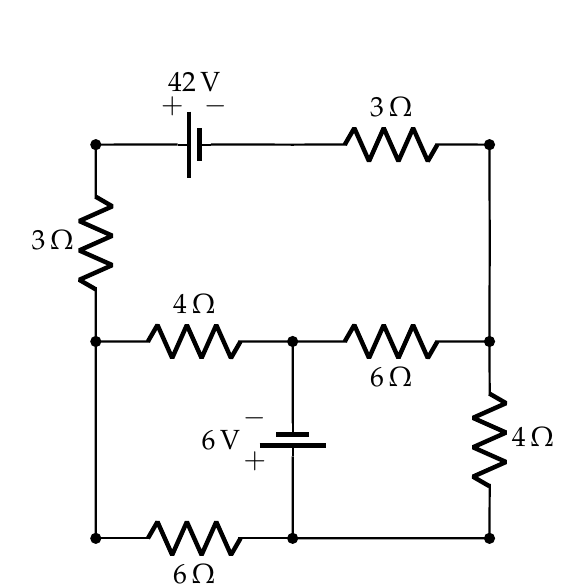
\begin{tikzpicture}[american voltages,scale=1.25]
      \draw[thick](0,0) to[short,*-](0,2) to[R=3<\ohm>,*-] (0,4)
      to[battery1=42<\volt>,*-](2,4) to[R=3<\ohm>] (4,4) to[short,*-](4,2)
      to[R=4<\ohm>,*-](4,0) to[short,*-](2,0) to[battery1=6<\volt>,*-](2,2)
      to[R,l_=4<\ohm>,*-](0,2);
      \draw[thick](0,0) to[R,l_=6<\ohm>](2,0);
      \draw[thick](2,2) to[R,l_=6<\ohm>](4,2);
    \end{tikzpicture}
  \end{center}
  \newpage
  
\item The capacitor in the circuit is initially uncharged. Find the current
  through the battery
  \begin{enumerate}[noitemsep]
  \item Immediately after the switch is closed
  \item A long time after the switch is closed 
  \end{enumerate}

  \begin{center}
    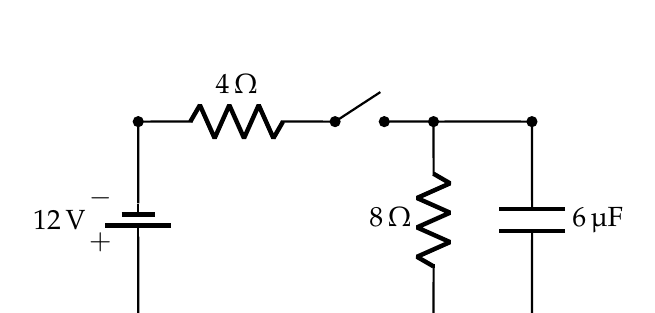
\begin{tikzpicture}[scale=1.25,american voltages]
      \draw[thick] (0,0) to[battery1=12<\volt>,*-*] (0,2) to[R=4<\ohm>] (2,2)
      to[short,*-](2.46,2.3);
      \draw[thick](2.5,2) to[short,*-*] (3,2) to[short,-*] (4,2)
      to[C=6<\micro\farad>,-*] (4,0)--(0,0);
      \draw[thick] (3,0) to[R=8<\ohm>,*-] (3,2);
    \end{tikzpicture}
  \end{center}


\end{enumerate}


\end{document}
